\documentclass{article}
\usepackage{spconf,amsmath,graphicx}

\newcommand{\figref}[1]{Figure~\ref{fig:#1}}

% Example definitions.
% --------------------
\def\x{{\mathbf x}}
\def\L{{\cal L}}

% Title.
% ------
\title{Deep Methods for Estimating Transient Scene Properties}
%
% Single address.
% ---------------
\name{}
\address{University of Kentucky}
%
% For example:
% ------------
%\address{School\\
%	Department\\
%	Address}
%
% Two addresses (uncomment and modify for two-address case).
% ----------------------------------------------------------
%\twoauthors
%  {A. Author-one, B. Author-two\sthanks{Thanks to XYZ agency for funding.}}
%	{School A-B\\
%	Department A-B\\
%	Address A-B}
%  {C. Author-three, D. Author-four\sthanks{The fourth author performed the work
%	while at ...}}
%	{School C-D\\
%	Department C-D\\
%	Address C-D}
%
\begin{document}
%\ninept
%
\maketitle
%
\begin{abstract}

  Deep learning has been used to obtain state of the art results in
  problems ranging from object classification, object detection, and
  scene classification. We evaluate the use of deep learning to
  predict more subtle visual scene aspects, such as the weather, the
  season, and subjective scene properties. 

\end{abstract}
%
\begin{keywords}
\end{keywords}

\section{Introduction}

% general intro to the problem and why it is important

% what do we propose to do? 

% how do we evaluate this? 
We evaluate the proposed method on several benchmarks 

% what we can do now that we have this?

% key contributions: repeat what was said above in bullet point form
The key contributions of this work are:
\begin{itemize}

  \item comparison of several deep learning network architectures for
    the problem

  \item state-of-the-art results on two benchmark datasets (transient
    attributes and two class weather)

  \item something with running it on webcam data?

\end{itemize}

\subsection{Related Work}

Previous approaches to this problem include (some general description
of previous approaches and how they compare to what we propose).

List of related papers:
\begin{itemize}

  \item add citation and one sentence description of what it does, one
    sentence description of how it is different from what we do, maybe
    something about how they evaluate.

\end{itemize}

\section{Estimating Transient Attributes Using CNNs}

\subsection{Recap of CNNs}

TODO: add a summary of the different models, and how they were
trained, include a bibtex citation for each one.

\subsection{Description of how we train ours}

TODO: write me\newline 
(This could change. Connor is training on the random split right now
to see how well we do)
\newline\indent
We finetuned the last layer of each of the networks using the holdout 
split in the transient attributes dataset.  This train/test split uses
the data from 81 webcams for training and the data from 20 separate 
webcams for testing.  Data from webcams in the training set does not
appear in the testing set using the holdout split.  This is contrary to 
the random train/test split.  

\subsection{Deep Network Visualization}

TODO: pictures of what the network looks like\dots highlighting how it
is different from those trained for other purposes... probably
focusing on the one or two that work the best

\section{Evaluation}
\indent
\figref{sort} shows the average errors from Caffenet for each attribute
in a sorted graph.  The attributes where Caffenet performed best are towards
the left side of the graph and the attributes where Caffenet performed
worst are on the right side of the graph. \figref{relerr} and \figref{compare} 
compare this performance to the performance of \cite{Laffont14}.
\newline\indent
\figref{compare} shows the average errors from Caffenet and \cite{Laffont14}
for each attribute in the dataset.  The green bars represent the average errors
from \cite{Laffont14} and the blue bars represent the average errors from Caffenet.
As \figref{relerr} shows as well, Caffenet performs better on more than half of 
the attributes.  Caffenet has a lower average error for most of these attributes.
\newline\indent
\figref{relerr} shows the relative error between our method using Caffenet
and the method presented in \cite{Laffont14}.  The average relative error 
for each attribute using the method in \cite{Laffont14} was subtracted from
the average relative error using Caffenet.  A negative value means Caffenet
had a smaller error and a positive value means \cite{Laffont14} had a smaller
error.  For example, the difference between the two methods on the attribute
night was around 3.2 percentage points, with Caffenet having the smaller 
error. 
 
%Suggested plots:
%\begin{itemize}
%
%  \item summary results you have already shown
%
%  \item example good results, and plausible bad results
%
%\end{itemize}


\begin{figure}[t]
	\centering
		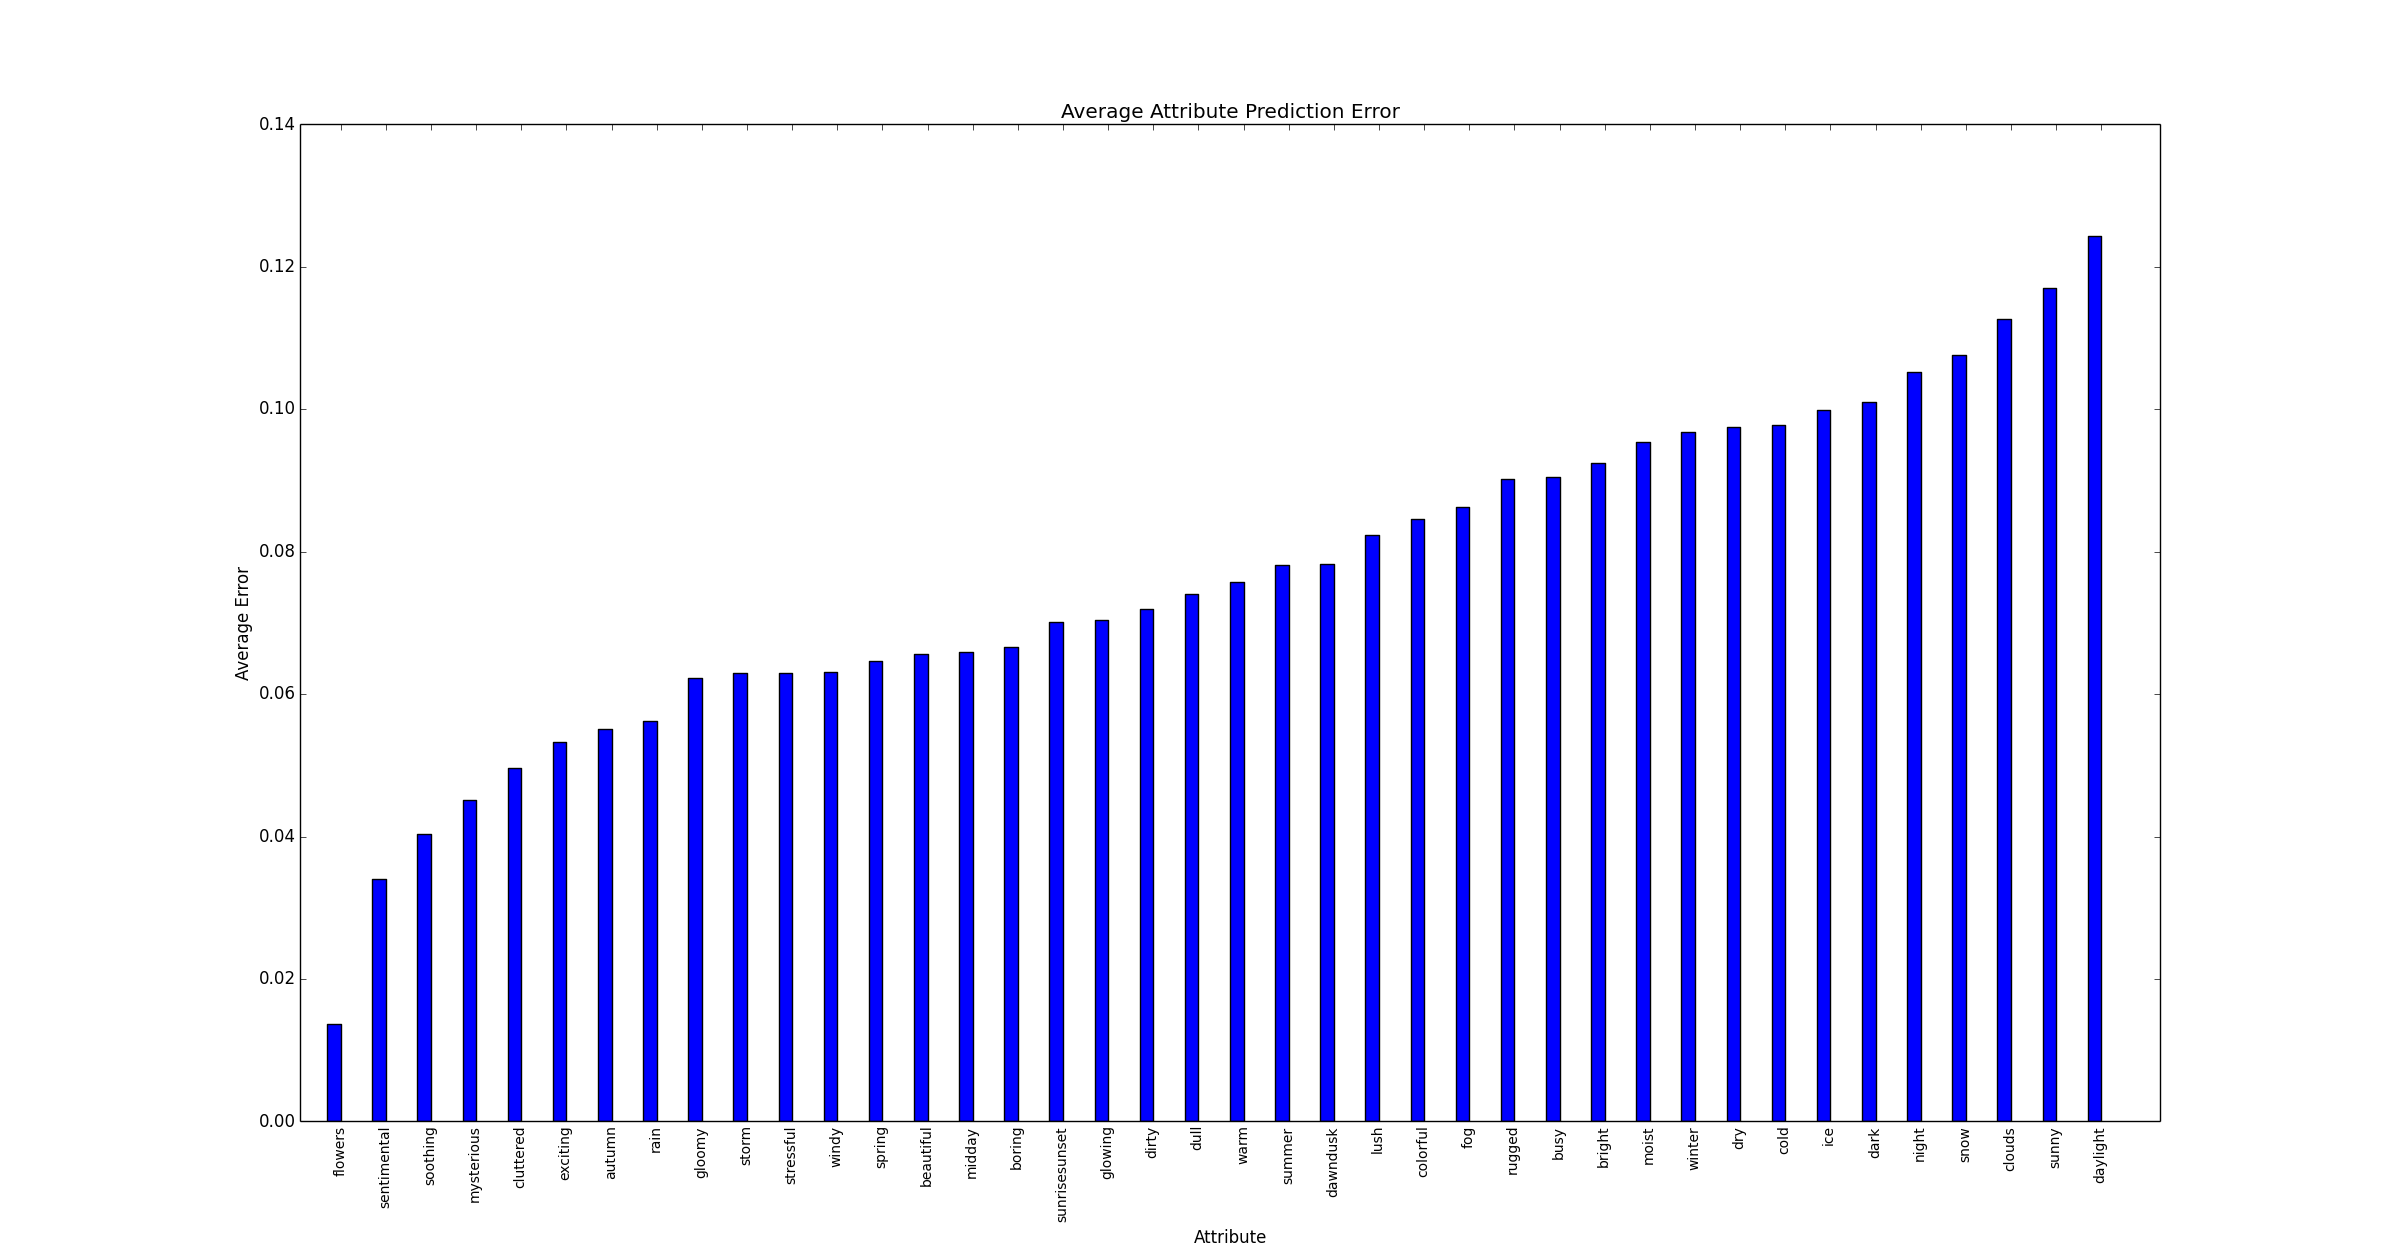
\includegraphics[width=0.5\textwidth]{figs/caffenet_avg_err.png}
		\caption{Sorted errors from caffenet}\label{fig:sort}
\end{figure}

\begin{figure}[t]
	\centering
		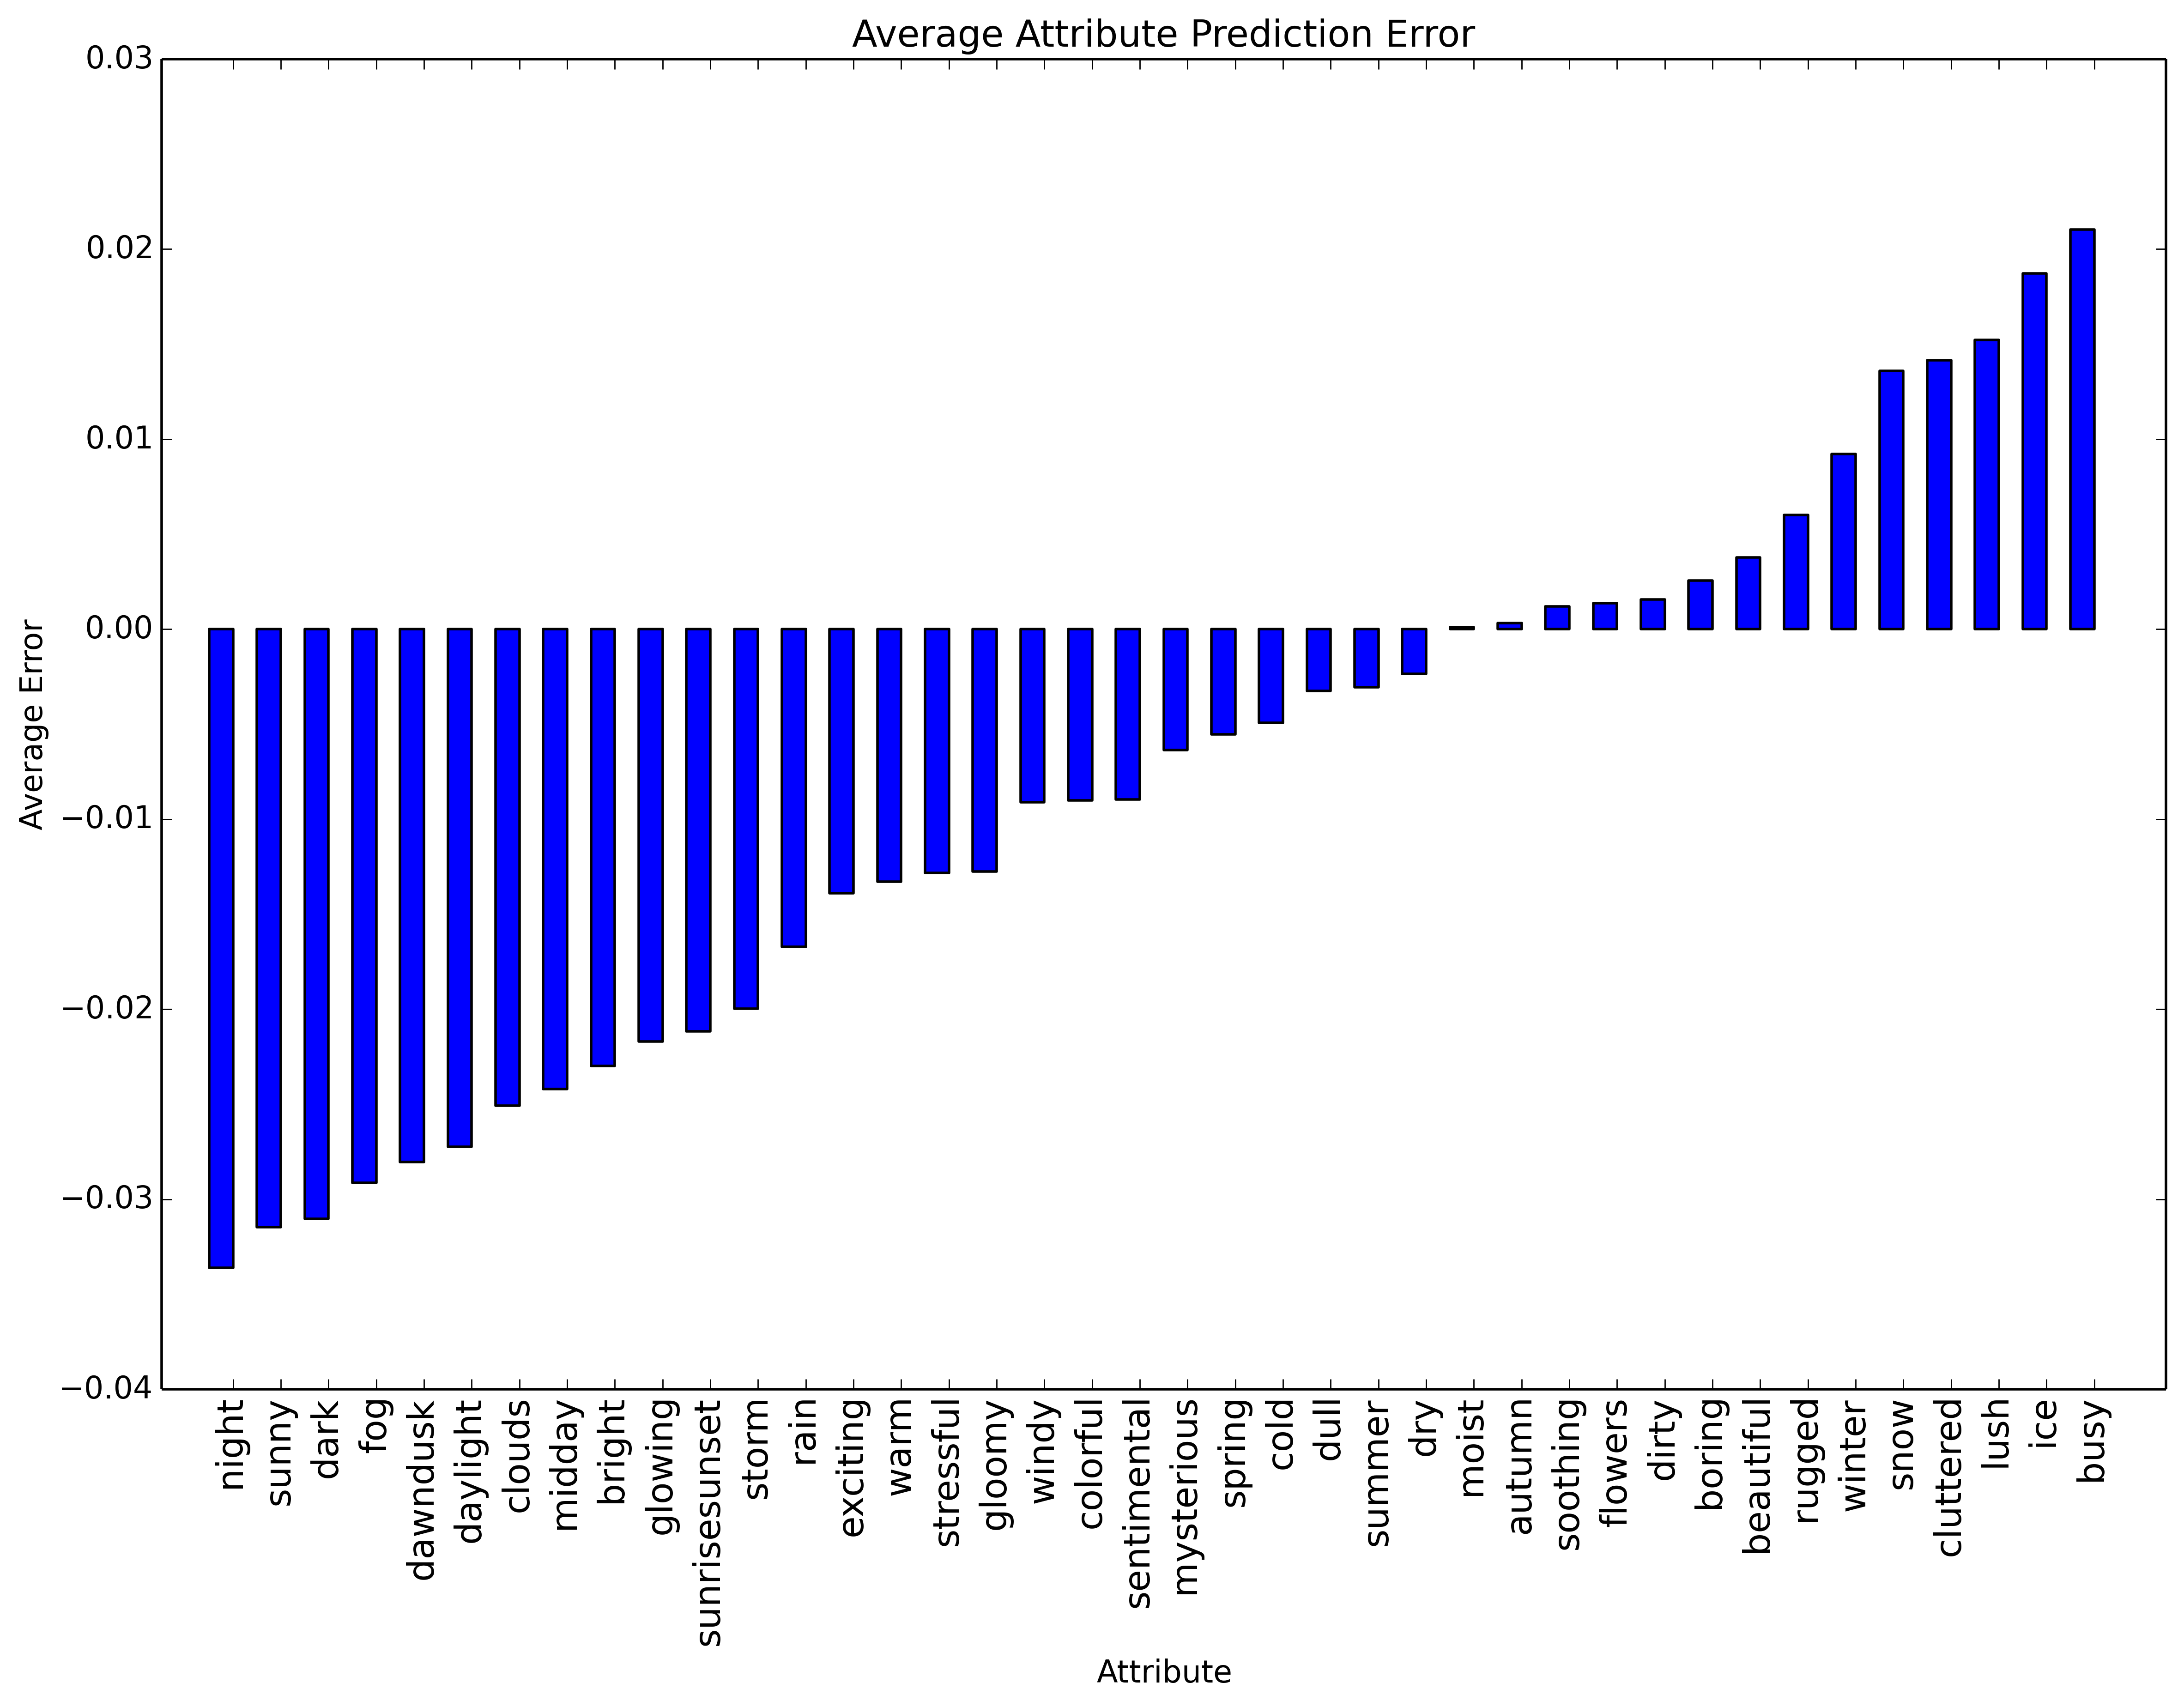
\includegraphics[width=0.5\textwidth]{figs/rel_err_tight.png}
		\caption{Relative errors us minus them}\label{fig:relerr}
\end{figure}

\begin{figure}[t]
	\centering
		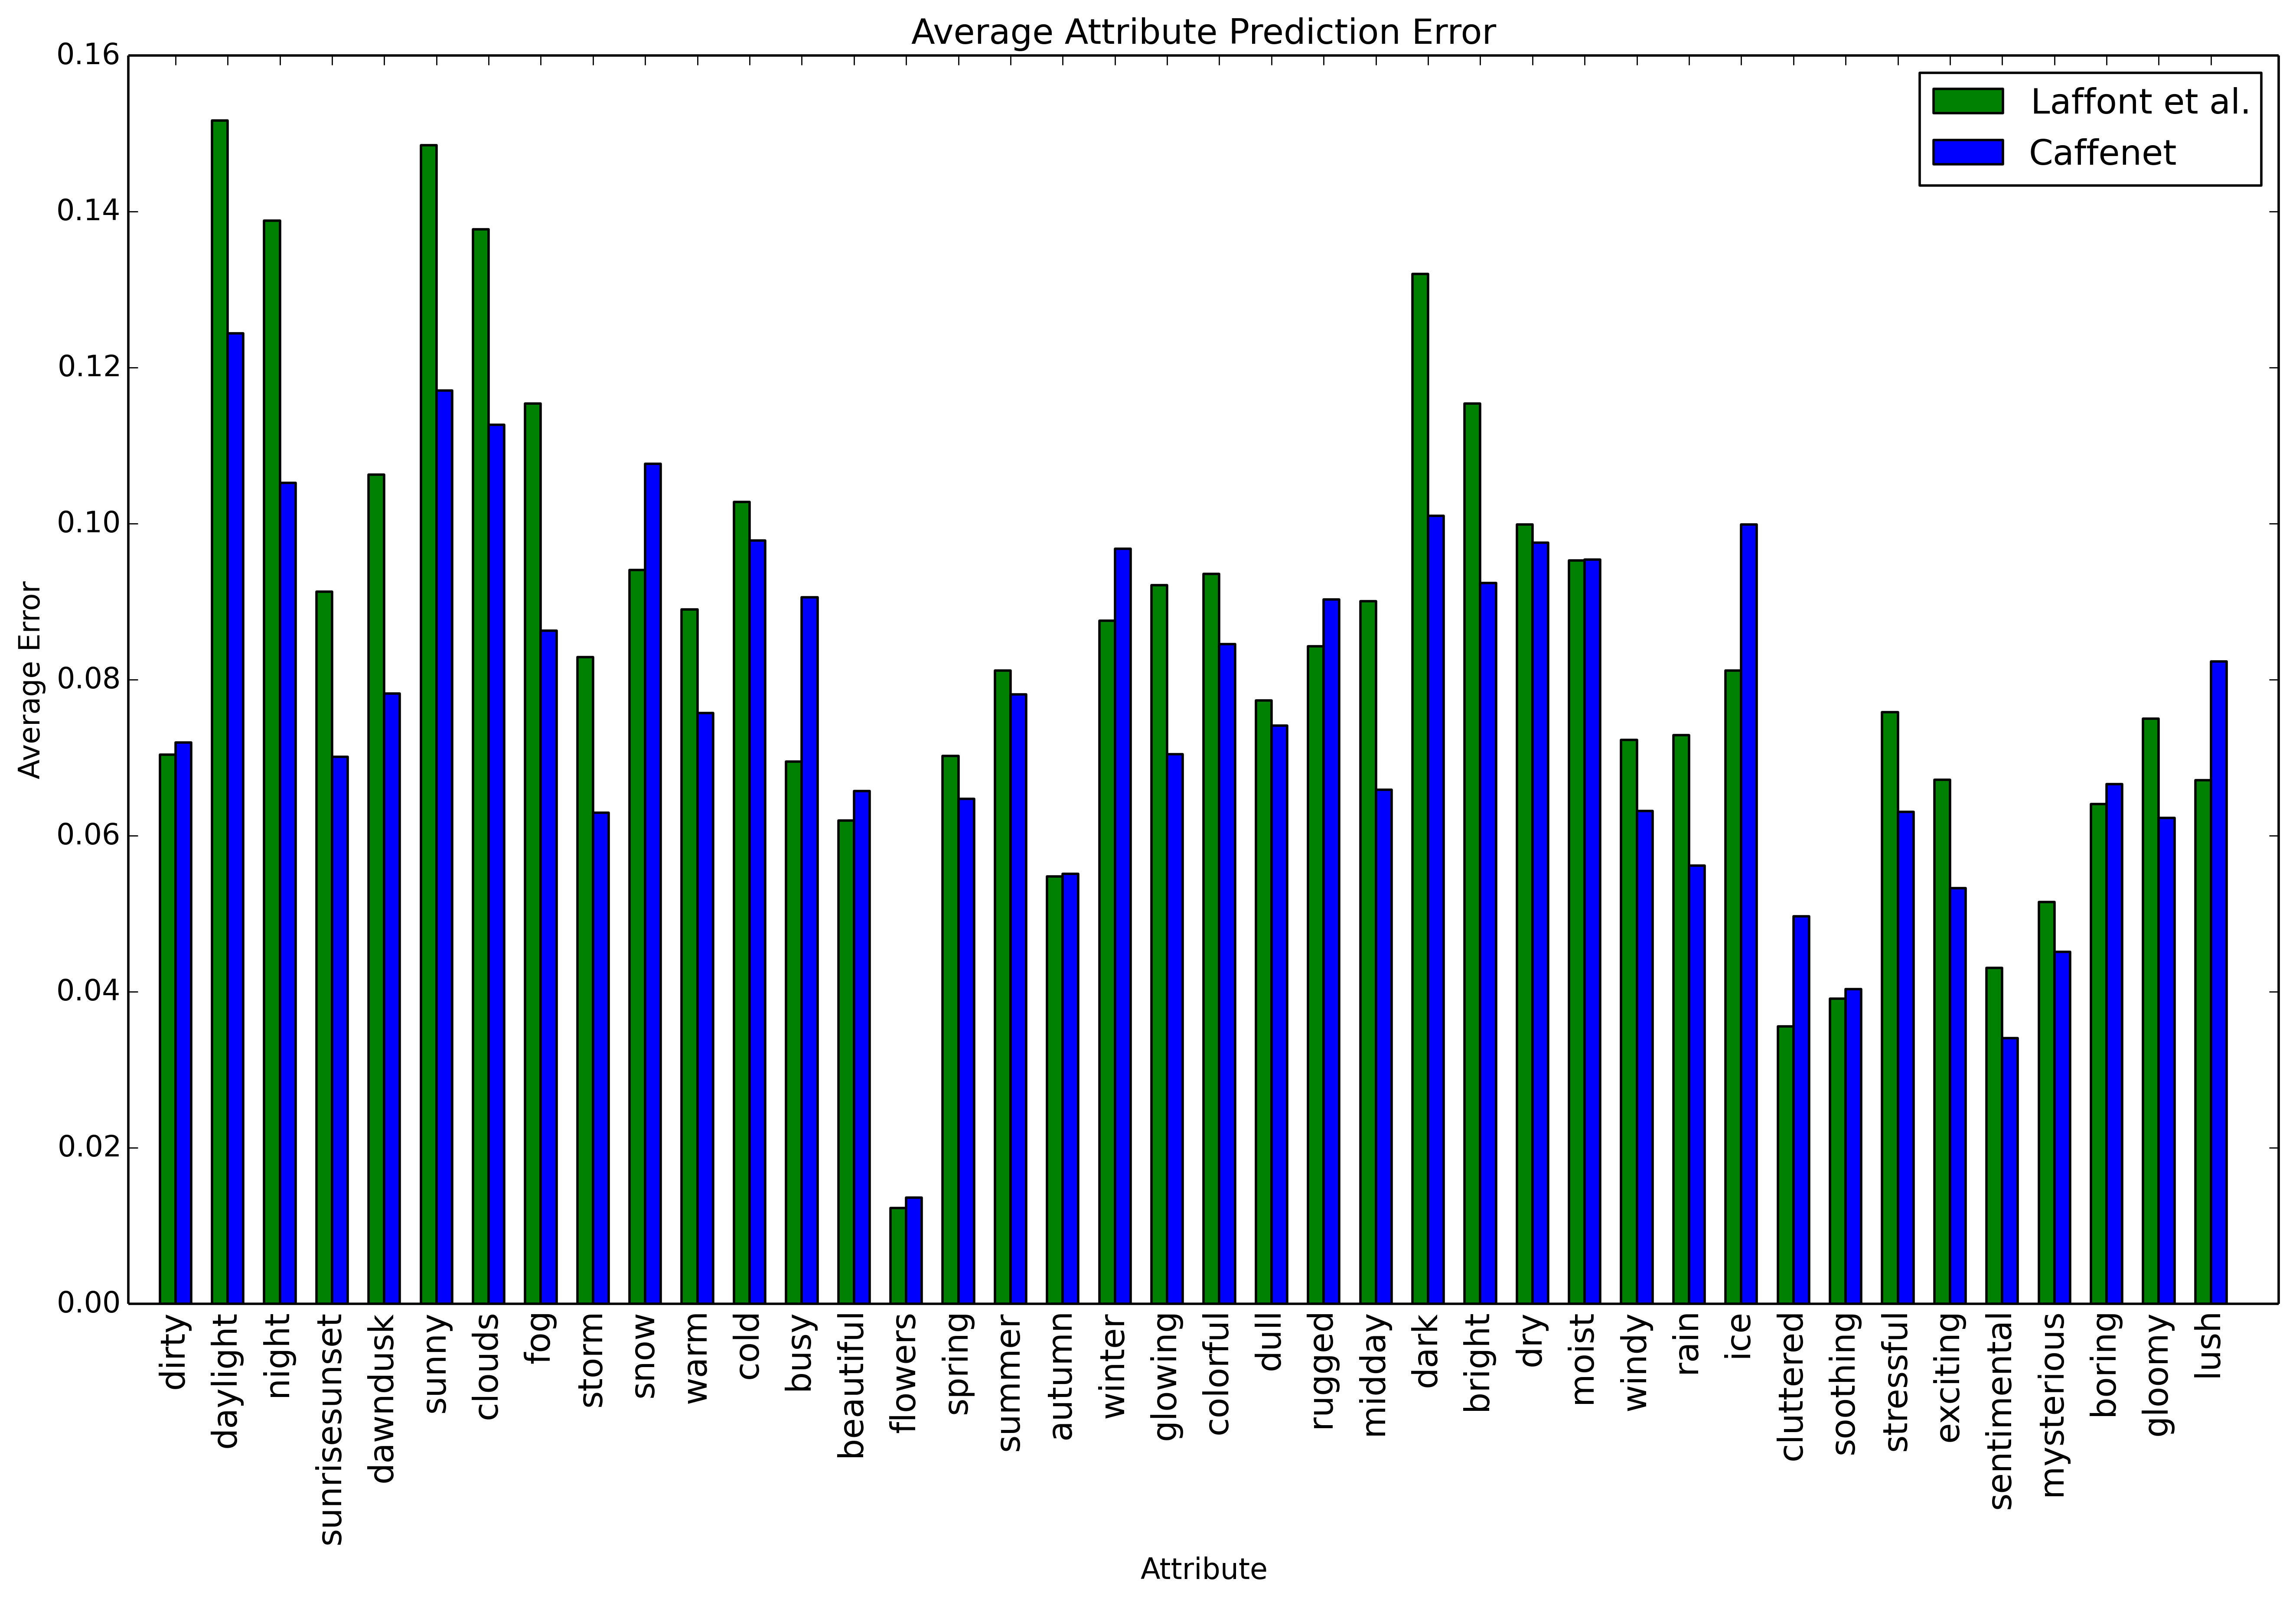
\includegraphics[width=0.5\textwidth]{figs/avg_err_compare_tight.png}
		\caption{comparing average errors}\label{fig:compare}
\end{figure}

\begin{figure*}[t]
	\centering
		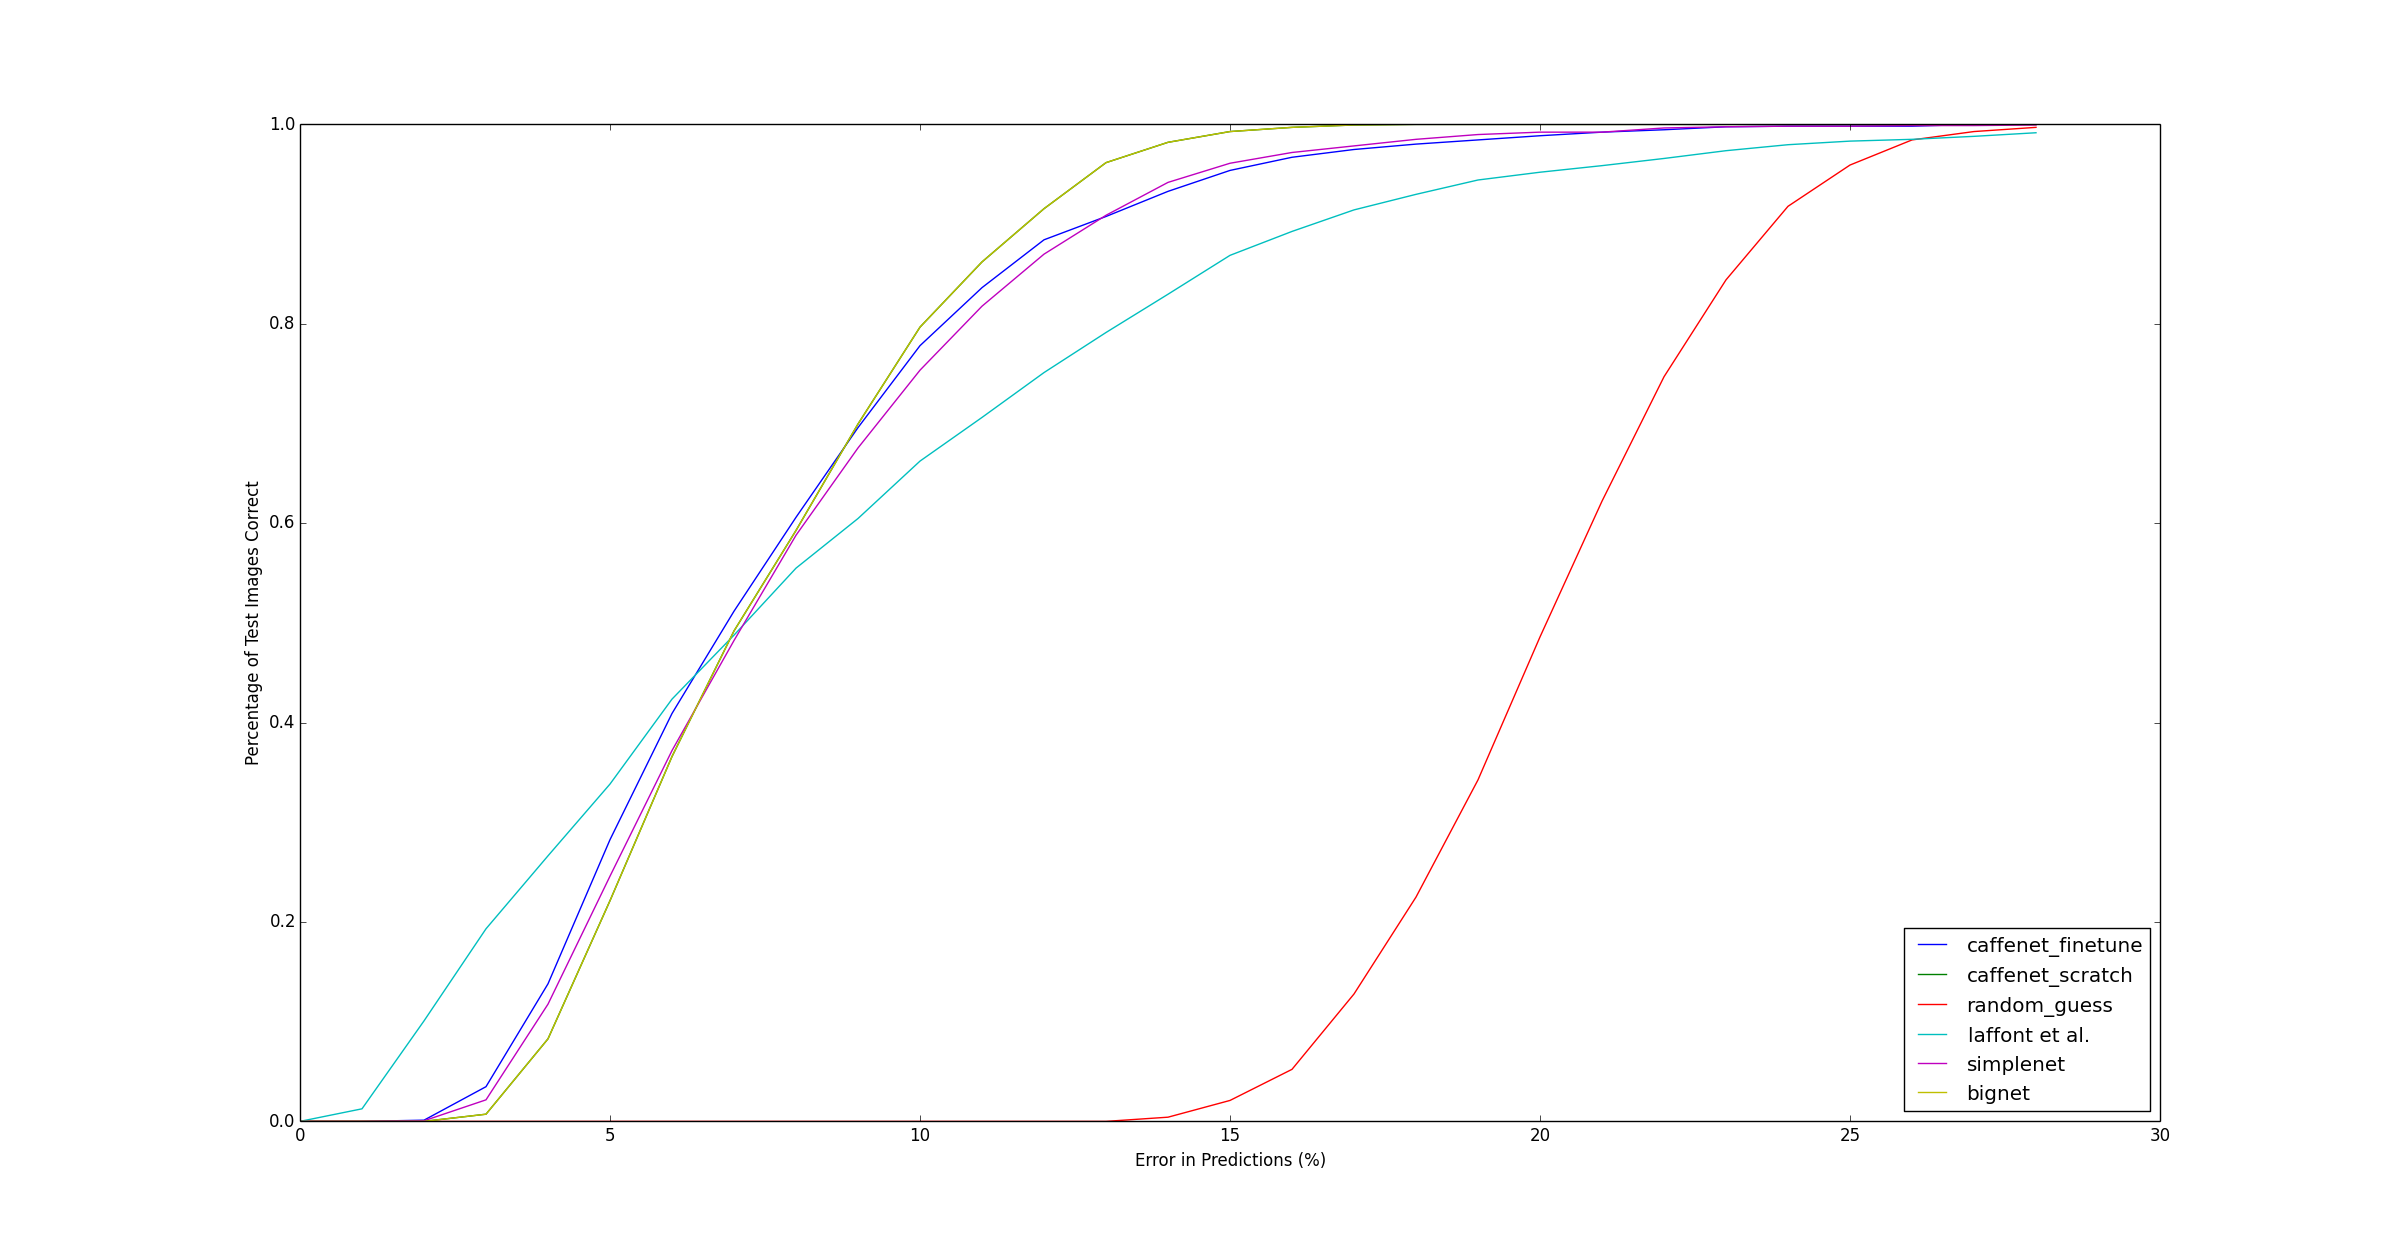
\includegraphics[width=1.0\textwidth]{figs/fig_1.png}
		\caption{These are some evaluation curves. needs to be full top page}
\end{figure*}

\section{Conclusions}

TODO: write me

more accurate

simpler and easier to train

faster

composable

\bibliographystyle{IEEEbib}
\bibliography{refs}

\end{document}

